% !TEX program = xelatex
% !TEX encoding = UTF-8
% !BIB program = bibtex
% !TEX spellcheck = en_US
\documentclass[12pt]{article}
\usepackage[letterpaper, margin=1in]{geometry}
\usepackage{amsmath,amssymb}
\usepackage{graphicx}
\usepackage{subfigure}
\usepackage{newpxtext,newpxmath}
\usepackage{siunitx}
\usepackage{hyperref}
\usepackage{bm}
\usepackage[version=4]{mhchem}
\usepackage{tikz}
\usetikzlibrary{calc}
\usetikzlibrary{arrows.meta}
\usetikzlibrary{decorations.pathreplacing}
\usepackage{relsize}
\tikzset{fontscale/.style = {font=\relscale{#1}}
}
\usepackage{wrapfig}
\usepackage{lipsum}

\makeatletter
\newcommand{\gettikzxy}[3]{%
  \tikz@scan@one@point\pgfutil@firstofone#1\relax
  \edef#2{\the\pgf@x}%
  \edef#3{\the\pgf@y}%
}
\makeatother

\title{Spinodal Decomposition}
\author{}
\date{}

\begin{document}
\maketitle

Consider a binary alloy system with a miscibility gap,
i.e.,
\begin{figure}[h]
	\begin{minipage}[l]{0.3\textwidth}
		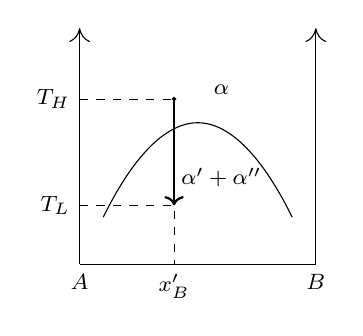
\begin{tikzpicture}[scale=3, font=\footnotesize]
	% axis
	\draw [-{>[scale=2.5,
    length=2,
    width=3]}] (0,0) -- (0,1);
	\draw (0,0) -- (1,0);
	\draw [-{>[scale=2.5,
    length=2,
    width=3]}] (1,0) -- (1,1);

	% curve
	\coordinate (A) at (0.1,0.2);
	\coordinate (B) at (0.9,0.2);
	\draw (A) parabola[bend pos=0.5] bend +(0,0.4) (B);

	% line
	\coordinate (xb') at (0.4,0);
	\coordinate (TL) at (0,0.25);
	\coordinate (TH) at (0, 0.7);
	\draw[dashed] (TL) -| (xb');
	\draw[dashed] (TH) -- ($ (xb') + (TH) $);

	% arrow
	\draw[->, thick] ($ (xb') + (TH) $) -- ($ (xb') + (TL) $);

	% point
	\draw[fill=black] ($ (xb') + (TH) $) circle[radius=0.2pt];

	% text
	\draw (TH) node[anchor=east] {$T_H$};
	\draw (TL) node[anchor=east] {$T_L$};
	\draw (0.6,0.45) node[anchor=north] {$\alpha'+\alpha''$};
	\draw (0.6,0.8) node[anchor=north] {$\alpha$};
	\draw (xb') node[anchor=north] {$x_B'$};
	\draw (0,0) node[anchor=north] {$A$};
	\draw (1,0) node[anchor=north] {$B$};
\end{tikzpicture}
	\end{minipage}%
	\hfil
	\begin{minipage}[r]{0.6\textwidth}
		now, consider a transformation which must occur when an alloy
		with composition $x_B'$ is quenched from temperature $T_H$
		to a lower temperature $T_L$', i.e.,
    \begin{equation*}
      \ce{$\alpha$ -> $\alpha' + \alpha''$}.
    \end{equation*}
	\end{minipage}
\end{figure}

In order to properly deal with the transformation, we need to analyze,
not surprisingly, the $G_{\text{sol}}$ vs composition relation at the
transformation temperature $T_L$!

I.e.,
\begin{figure}[h]
	\begin{minipage}[l]{0.3\textwidth}
		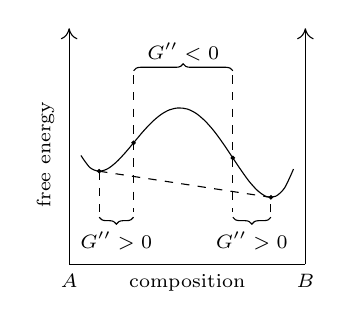
\begin{tikzpicture}[scale=3, domain=0.05:0.95, font=\scriptsize]
	% axis
	\draw [-{>[scale=2,
			length=2,
			width=3]}] (0,0) -- (0,1);
	\draw (0,0) -- (1,0);
	\draw [-{>[scale=2,
			length=2,
			width=3]}] (1,0) -- (1,1);

	\begin{scope}[yscale=0.5, yshift=0.5cm]
		% curve
		\coordinate (g00A) at (0.272815, 0.529808);
		\coordinate (g00B) at (0.692895, 0.402102);
		\coordinate (g0A) at (0.127138, 0.289339);
		\coordinate (g0B) at (0.854233, 0.0681958);
		\draw plot[smooth] (\x, {0.7 - 7.45598 * \x + 41.666 * \x^2 - 70.9531 * \x^3 + 36.7362 * \x^4});
	\end{scope}


	% line
	\gettikzxy{(g00A)}{\ax}{\ay};
	\gettikzxy{(g00B)}{\bx}{\by};
	\gettikzxy{(g0A)}{\fax}{\fay};
	\gettikzxy{(g0B)}{\fbx}{\fby};
	\draw[dashed] (\ax, 0.8) -- (\ax, 0.22);
	\draw[dashed] (\bx, 0.8) -- (\bx, 0.22);
	\draw[dashed] (g0A) -- (g0B);
	\draw[dashed] (\fax, \fay) -- (\fax, 0.22);
	\draw[dashed] (\fbx, 0.22) -- (\fbx, \fby);

	% point
	\draw[fill=black] (g00A) circle[radius=0.2pt];
	\draw[fill=black] (g00B) circle[radius=0.2pt];
	\draw[fill=black] (g0A) circle[radius=0.2pt];
	\draw[fill=black] (g0B) circle[radius=0.2pt];

	% text
	\draw (0.5, 0) node[anchor=north] {composition};
	\draw (0,0) node[anchor=north] {$A$};
	\draw (1,0) node[anchor=north] {$B$};
	\draw (-0.1,0.2) node[anchor=west, rotate=90] {free energy};
	\draw ($ ( {(\ax + \bx)/2}, 0.9) $) node (g) {$G'' < 0$};  % You need to wrap the expression into { } to hide the second pair of ( ) from the TeX parser.
	\draw ($ ( {(\fax + \ax)/2}, 0.1) $) node (g) {$G'' > 0$};
	\draw ($ ( {(\fbx + \bx)/2}, 0.1) $) node (g) {$G'' > 0$};

	% others
	\draw [
		decoration={
				brace
			},
		decorate
	] (\ax,0.82) -- (\bx,0.82);
	\draw [
		decoration={
				brace,
				mirror,
			},
		decorate
	] (\fax, 0.2) -- (\ax, 0.2);
	\draw [
		decoration={
				brace,
			},
		decorate
	] (\fbx, 0.2) -- (\bx, 0.2);
\end{tikzpicture}
	\end{minipage}%
	\hfil
	\begin{minipage}[r]{0.6\textwidth}
	 In particular,
   \begin{enumerate}
     \item If $x_B'$ inside the $G''<0$ region, then small fluctuations
     in composition $\Rightarrow G \downarrow$ about $x_B'$.
     $\therefore$ system is unstable and decomposition continues via
     ``uphill'' diffusion!
   \end{enumerate}
	\end{minipage}
\end{figure}

\end{document}
